%%%%%%%%%%%%%%%%%%%%%%%%%%%%%%%%%%%%%%%%%%%%%%%%%%%%%%%%%%%%%%%%%%%%%%%%%%%%%%%
%%                                                                           %%
%%   Dr Derek Harter                                                         %%
%%   Profesor, Department of Computer Science                                %% 
%%   Texas A&M University - Commerce, USA                                    %%
%%                                                                           %%
%%%%%%%%%%%%%%%%%%%%%%%%%%%%%%%%%%%%%%%%%%%%%%%%%%%%%%%%%%%%%%%%%%%%%%%%%%%%%%%
%%%%     SETTING STARTS - DO NOT CHANGE Unless your TeX setting require so   %%
%%%%%%%%%%%%%%%%%%%%%%%%%%%%%%%%%%%%%%%%%%%%%%%%%%%%%%%%%%%%%%%%%%%%%%%%%%%%%%%
%%----------------------------------------------------------------------------------
% DO NOT Change this. It is the required setting letterpaper page, 11pt, onside print, book style
%%----------------------------------------------------------------------------------
\documentclass[letterpaper,11pt,oneside]{book}

%%-------------------------------------
%% Page margin settings - % half inch margin all sides (recommended)
%%-------------------------------------
\usepackage[margin=1.2in]{geometry} 

%%-------------------------------------
%% Font settings - % CM San or Ariel (recommended)
%%-------------------------------------
% Switch the following two line off: to revert back to default LaTex font (NOT recommended)
\usepackage{amsfonts}
\renewcommand*\familydefault{\sfdefault}

%%-------------------------------------
%% Math/Definition/Theorem/Algorithm packages settings 
%%-------------------------------------
\usepackage[cmex10]{amsmath}
\usepackage{amssymb}
\usepackage{amsthm}
\newtheorem{mydef}{Definition}
\newtheorem{mytherm}{Theorem}

%%-------------------------------------
%% Algorithms/Code Listing environment settings  - 
%% Please do not change these settings
%%-------------------------------------
\usepackage{algorithm}
\usepackage{algpseudocode}
\renewcommand{\algorithmicrequire}{\textbf{Input:}}
\renewcommand{\algorithmicensure}{\textbf{Output:}}
\usepackage[utf8]{inputenc}
\usepackage{listings}
\usepackage{xcolor}
\definecolor{codegreen}{rgb}{0,0.6,0.1}
\definecolor{codegray}{rgb}{0.5,0.5,0.5}
\definecolor{codeblue}{rgb}{0.10,0.00,1.00}
\definecolor{codepurple}{rgb}{0.58,0,0.82}
\definecolor{backcolour}{rgb}{1.0,1.0,1.0}

\lstdefinestyle{mystyle}{
    backgroundcolor=\color{backcolour},   
    commentstyle=\color{codegreen},
    keywordstyle=\color{codeblue},
    numberstyle=\tiny\color{codegray},
    stringstyle=\color{codepurple},
    basicstyle=\ttfamily\footnotesize,
    breakatwhitespace=false,         
    breaklines=true,                 
    captionpos=b,                        
    keepspaces=true,                 
    numbers=left,                    
    numbersep=5pt,                  
    showspaces=false,                
    showstringspaces=false,
    showtabs=false,                  
    tabsize=2,
    frame=none
}
\lstset{style=mystyle}

%%-------------------------------------
%% Graphics/Figures environment settings
%%-------------------------------------
\usepackage{graphicx}
\usepackage{subfigure}
\usepackage{caption}
\usepackage{lipsum}

%%-------------------------------------
%% Table environment settings
%%-------------------------------------
\usepackage{multirow}
\usepackage{rotating}
\usepackage{makecell}
\usepackage{booktabs}
%\usepackage{longtable,booktabs}

%%-------------------------------------
%% List of Abbreviations settings
%%-------------------------------------
\usepackage{enumitem}
\newlist{abbrv}{itemize}{1}
\setlist[abbrv,1]{label=,labelwidth=1in,align=parleft,itemsep=0.1\baselineskip,leftmargin=!}

%%-------------------------------------
%% Bibliography/References settings   - Harvard Style was used in this report
%%-------------------------------------
\usepackage[hidelinks]{hyperref}
\usepackage[comma,authoryear]{natbib}
\renewcommand{\bibname}{References} % DO NOT remove or switch of 

%%-------------------------------------
%% Appendix settings     
%%-------------------------------------
\usepackage[toc]{appendix}
%%%%%%%%%%%%%%%%%%%%%%%%%%%%%%%%%%%%%%%%%%%%%%%%%%%%%%%%%%%%%%%%%%%%%%%%%%%%%%%%%%%%%%%
%%%%                     SETTING ENDS                                            %%%%%%
%%%%%%%%%%%%%%%%%%%%%%%%%%%%%%%%%%%%%%%%%%%%%%%%%%%%%%%%%%%%%%%%%%%%%%%%%%%%%%%%%%%%%%%
\begin{document}

    \captionsetup[figure]{margin=1.5cm,font=small,name={Figure},labelsep=colon}
    \captionsetup[table]{margin=1.5cm,font=small,name={Table},labelsep=colon}
    \SetLipsumDefault{1}
    
    \frontmatter
    
    \begin{titlepage}      
        \begin{center}
            
\includegraphics[width=3cm]{figures/tamuc-logo.png}\\[0.5cm]
            {\LARGE Texas A\&M University - Commerce\\[0.5cm]
            Department of Computer Science}\\[2cm]
			%{\color{blue} \rule{\textwidth}{1pt}}
			
			% -------------------------------
			% You need to edit some details here
			% -------------------------------  
            \linespread{1.2}\huge {
                %%%%%%%%%%%%%%%%%%%%%%%%%%%%
                %TODO: 1 TITLE of Your PROJECT 
                %%%%%%%%%%%%%%%%%%%%%%%%%%%%
                % chnage the following line                
                Performance Analysis of LR and SVM - Supervised Machine Learning Algorithms for Diabetes Prediction
            
            }
            \linespread{1}~\\[2cm]
			%{\color{blue} \rule{\textwidth}{1pt}}
            {\Large 
                %%%%%%%%%%%%%%%%%%%%%%%%%%%%
                %TODO: 2 YOUR NAME
                %%%%%%%%%%%%%%%%%%%%%%%%%%%%             
                % chnage the following line
                Vyshnavi Sanikommu
                % change end             
            }\\[1cm] 
            

            {\large 
                %%%%%%%%%%%%%%%%%%%%%%%%%%%%
                %TODO: 3 YOUR NAME Supervisor's name(s)
                %%%%%%%%%%%%%%%%%%%%%%%%%%%%             
                % change the following line                
                \emph{Supervisor:} Derek Harter, Ph.D.}\\[1cm] % if applicable
            
    		% PLEASE DO NOT CHANGE THIS TEXT %
            \large A report submitted in partial fulfilment of the requirements of\\Texas A\&M University - Commerce for the degree of\\ Master of Science in \textit{Computer Science}\\[0.3cm] 
            \vfill
            
            
            \today % Please update this date you can use \date{April 2020} for fixed date
        \end{center}
    \end{titlepage}
    
    
    % -------------------------------------------------------------------
    % Declaration
    % -------------------------------------------------------------------
    \newpage
    \thispagestyle{empty}
    \chapter*{\Large Declaration}
    % PLEASE CHANGE THIS TEXT EXCEPT YOUR NAME%
    % -------------------------------
    %TODO: PLEASE ONLY UPDATE HERE -- PLEASE WRITE YOUR NAME %    
    % ------------------------------- 
    I,
    %%%%%%%%%%%%%%%%%%%%%%%
     Vyshnavi Sanikommu, % Mandatory part
    %%%%%%%%%%%%%%%%%%%%%%%
    of the Department of Computer Science, Texas A\&M University - Commerce, confirm that this is my own work and figures, tables, equations, code snippets, artworks, and illustrations in this report are original and have not been taken from any other person's work, except where the works of others have been explicitly acknowledged, quoted, and referenced. I understand that if failing to do so will be considered a case of plagiarism. Plagiarism is a form of academic misconduct and will be penalised accordingly. \\
    
    %% Please delete as appropriate. 
    \noindent
    %%%%%%%%%%%%%%%%%%%%%%%%%%%%%%%%%%%%%%%%%%%%%%% 
    %TODO 1 Consent for example copy -  we will use 
    I give consent to a copy of my report being shared with future students as an exemplar. \\
    
    \noindent
    %%%%%%%%%%%%%%%%%%%%%%%%%%%%%%%%%%%%%%%%%%%%%%% 
    %TODO 2 Consent to let the report to use use by library for public use
    I give consent for my work to be made available more widely to members of TAMUC and public with interest in teaching, learning and research. 
    %%%%%%%%%%%%%%%%%%%%%%%%%%%%%%%%%%%%%%%%%%%%%%%
    ~\\[1cm]
    \begin{flushright}
	%------------------------------ 
	% change the following line
    %TODO: PLEASE UPDATE  Your Name  -------------------------------%
	Vyshnavi Sanikommu % Please change it to your name
    
    \today
    \end{flushright}

     
    % -------------------------------------------------------------------
    % Abstract and Acknowledgement
    % -------------------------------------------------------------------
    
    %Two resources useful for abstract writing.
% Guidance of how to write an abstract/summary provided by Nature: https://cbs.umn.edu/sites/cbs.umn.edu/files/public/downloads/Annotated_Nature_abstract.pdf %https://writingcenter.gmu.edu/guides/writing-an-abstract
\chapter*{\center \Large  Abstract}
%%%%%%%%%%%%%%%%%%%%%%%%%%%%%%%%%%%%%%
% Replace all text with your text
%%%%%%%%%%%%%%%%%%%%%%%%%%%%%%%%%%%

Diabetes is one of the most lethal diseases in the world. According to International Diabetes Foundation 537 million people are living with diabetes across the world. By 2045, this would be 783 million. Diabetes is a disease caused due to an increase in blood glucose level. High blood glucose produces the symptoms of frequent urination, increased hunger, and thirst. Diabetes is a leading cause of blindness, kidney failure, amputations, heart failure and stroke. When we eat, our body converts the food into sugars, or glucose. The pancreas releases insulin, a crucial hormone that unlocks cells to facilitate glucose entry. This mechanism enables our cells to utilize glucose as an energy source, supporting essential bodily functions. Machine learning is an emerging scientific field in data science dealing with the ways in which machines learn from experience. The aim of this project is to develop a system which can perform early prediction of diabetes for a patient with a higher accuracy by combining the results of supervised machine learning algorithms like logistic regression and support vector machine. Machine learning techniques provide better results for prediction by constructing models from datasets collected from patients. The accuracy of the model using each of the algorithms is calculated by considering the meta parameters to achieve the best performance. Then the one with a good accuracy is taken as the model for predicting diabetes.



%%%%%%%%%%%%%%%%%%%%%%%%%%%%%%%%%%%%%%%%%%%%%%%%%%%%%%%%%%%%%%%%%%%%%%%%%s
~\\[1cm]
\noindent % Provide your key words
\textbf{Keywords:} Diabetes, Machine Learning, Logistic Regression, Support Vector Machine, Accuracy


    % -------------------------------------------------------------------
	% Acknowledgement
	% -------------------------------------------------------------------
   
    \chapter*{\center \Large  Acknowledgements}
%%%% Update with your text %%%%%%%%%%%%%%%
An acknowledgements section is optional. You may like to acknowledge the support and help of your supervisor(s), friends, or any other person(s), department(s), institute(s), etc. If you have been provided specific facility from department/school acknowledged so.  

   
    
    % -------------------------------------------------------------------
    % Contents, list of figures, list of tables
    % -------------------------------------------------------------------
    
    \tableofcontents
    \listoffigures
    \listoftables
    \chapter*{List of Abbreviations}
\chaptermark{List of Abbreviations}
%%%%%%%%%%%%%%%%%%%%%%%%%%%%%%%%%%%
%%  Enter your list of Abbreviation and Symbols in this file
%%%%%%%%%%%%%%%%%%%%%%%%%%%%%%%%%%%
\begin{abbrv}
    
    \item[SMPCS]			School of Mathematical, Physical and Computational Sciences
    
\end{abbrv}
 %  Enter your list of Abbreviation and Symbols in this file
    
    %%%%%%%%%%%%%%%%%%%%%%%%%%%%%%%%%%%%%%%%%%%%%%%%%%%%%%%%%%%%%%%%%%%%%%%%
    %%                                                                    %%  
    %%  Main chapters and sections of your project                        %%  
    %%  Everything from here on needs updates in your own words and works %%
    %%                                                                    %%
    %%%%%%%%%%%%%%%%%%%%%%%%%%%%%%%%%%%%%%%%%%%%%%%%%%%%%%%%%%%%%%%%%%%%%%%%
    \mainmatter
    % Read for preparation of document in LaTex 
    % Lamport, L. (1986), LATEX: A Document Preparation System, Addison-Wesley.
    
    \chapter{Introduction}
\label{ch:into} % This how you label a chapter and the key (e.g., ch:into) will be used to refer this chapter ``Introduction'' later in the report. 
% the key ``ch:into'' can be used with command \ref{ch:intor} to refere this Chapter.
Diabetes is a fast growing disease among the people even in youngsters nowadays. It is necessary to understand how it develops in our body. Firstly, we need to understand how a body works without diabetes. Sugar comes from the food that we eat, specially carbohydrates. When we eat this food, the body breaks them down to Sugars or Glucose. This glucose moves around the body in the bloodstream. This glucose was needed by body parts like brain, pancreas to function. The remainder of glucose is taken to the cells of our body and liver which is stored as energy for later use. In order to use glucose for our body, insulin is required which is a hormone generated by pancreas. Insulin is a key to a closed door which helps glucose moves from blood stream. If pancreas is not able to produce enough insulin or if our body cannot use insulin it produces then glucose levels increases in bloodstream which leads to diabetes.

~\\[0cm]
According to World Health Organization, diabetes is major cause of death worldwide. Around 422 million people worldwide have diabetes. Indeed, it caused deaths of 2 million people in 2019.

\section*{Types of Diabetes}
\textbf{Type 1} diabetes appear most often during childhood and characterized by the partial functioning of pancreas. The cells fail to produce sufficient amounts of Insulin. Initially, we do not see any symptoms as the pancreas remains partially functional. There is no proven study and known methods for prevention.

~\\[0cm]
\textbf{Type 2} diabetes affects how the body uses sugars for energy. The cells produce low quantity of insulin or the body stops using insulin which can lead to high levels of sugar in bloodstream. High levels of glucose in the bloodstream and urine referred as Diabetes Mellitus. It is most common type of diabetes found in many people. It is caused by genetic factors and the lifestyle. It affects older adults and more obese or overweight people.

~\\[0cm]
Early prediction of the disease can be controlled and save the life. To accomplish this, this work explores prediction of diabetes by taking various attributes related to diabetes disease. For this purpose, we use the Diabetes Dataset \cite{dataset} which has 2000 instances with 9 attributes - `Pregnancies`, `Glucose`, `BloodPressure`, `SkinThickness`, `Insulin`, `BMI`, `DiabetesPedigreeFunction`, `Age`, `Outcome` for creating classification models using logistic regression and support vector machine algorithms.



%%%%%%%%%%%%%%%%%%%%%%%%%%%%%%%%%%%%%%%%%%%%%%%%%%%%%%%%%%%%%%%%%%%%%%%%%%%%%%%%%%%
\section{Background}
\label{sec:into_back}
This study is undertaken to address the crucial need for accurate and reliable methods in predicting diabetes using logistic regression and support vector machine algorithms on patient data. The motivation behind this study stems from the growing significance of leveraging machine learning algorithms to assist medical professionals in diagnosing and managing diabetes. Predictive models based on patient data offer the potential to identify individuals at risk or in the early stages of diabetes, enabling proactive and personalized healthcare strategies. Algorithms - logistic regression and support vector machine are chosen due to their widespread use in medical data analysis and their capability to handle classification tasks. The study outcomes have practical implications for healthcare practitioners and researchers, offering insights into algorithm selection for accurate and interpret diabetes prediction.

%%%%%%%%%%%%%%%%%%%%%%%%%%%%%%%%%%%%%%%%%%%%%%%%%%%%%%%%%%%%%%%%%%%%%%%%%%%%%%%%%%%
\section{Research question}
\label{sec:intro_prob_art, linewidth:80}
This section provides a detailed exploration of the research problem. The main question is about understanding how accurate logistic regression and support vector machine are in predicting diabetes from patient's data. The focus is on figuring out what factors cause differences in accuracy, especially looking at the impact of hyper parameters.

%%%%%%%%%%%%%%%%%%%%%%%%%%%%%%%%%%%%%%%%%%%%%%%%%%%%%%%%%%%%%%%%%%%%%%%%%%%%%%%%%%%
\section{Aims and objectives}
\label{sec:intro_aims_obj}

The primary aim of this study is to assess and compare the predictive accuracy of logistic regression and support vector machine algorithms based on diabetic patient's data to decide if a patient is diabetic or not. This study aims to provide valuable insights into the strengths and limitations of these supervised machine learning approaches, contributing to the enhancement of diabetes prediction methodologies.

\textbf{Objectives:} 
The main objectives of this study is to do data processing, implement logistic regression and support vector machine models, hyper parameter tuning to achieve highest possible predictive accuracy. At the end, we will evaluate the performance of both classification models.

%%%%%%%%%%%%%%%%%%%%%%%%%%%%%%%%%%%%%%%%%%%%%%%%%%%%%%%%%%%%%%%%%%%%%%%%%%%%%%%%%%%
\section{Solution approach}
\label{sec:intro_sol} % label of Org section
Briefly describe the solution approach and the methodology applied in solving the set aims and objectives.

Depending on the project, you may like to alter the ``heading'' of this section. Check with you supervisor. Also, check what subsection or any other section that can be added in or removed from this template.

\subsection{A subsection 1}
\label{sec:intro_some_sub1}
You may or may not need subsections here. Depending on your project's needs, add two or more subsection(s). A section takes at least two subsections. 

\subsection{A subsection 2}
\label{sec:intro_some_sub2}
Depending on your project's needs, add more section(s) and subsection(s).

\subsubsection{A subsection 1 of a subsection}
\label{sec:intro_some_subsub1}
The command \textbackslash subsubsection\{\} creates a paragraph heading in \LaTeX.

\subsubsection{A subsection 2 of a subsection}
\label{sec:intro_some_subsub2}
Write your text here...

%%%%%%%%%%%%%%%%%%%%%%%%%%%%%%%%%%%%%%%%%%%%%%%%%%%%%%%%%%%%%%%%%%%%%%%%%%%%%%%%%%%
\section{Summary of contributions and achievements} %  use this section 
\label{sec:intro_sum_results} % label of summary of results
Describe clearly what you have done/created/achieved and what the major results and their implications are. 

    \chapter{Literature Review}
\label{ch:lit_rev} %Label of the chapter lit rev. The key ``ch:lit_rev'' can be used with command \ref{ch:lit_rev} to refer this Chapter.
The examination of relevant studies yields findings from various healthcare datasets, where researchers conducted analyses and predictions employing a range of methods and techniques. Numerous prediction models have been devised and applied by various researchers, utilizing different forms of data mining techniques, machine learning algorithms, or a combination of these methodologies.
% PLEAE CHANGE THE TITLE of this section
\section{Review of state-of-the-art} 
% Note the use of \cite{} and \citep{}
\cite{mujumdar2019diabetes} aims to create a system using machine learning algorithm and deep learning techniques to provide accurate results and reduce human efforts. The diabetes dataset contains 800 instances with 10 attributes. This study implemented various machine learning algorithms include Support Vector Classifier, Random Forest Classifier, Decision Tree Classifier, Extra Tree Classifier, Ada Boost algorithm, Perceptron, Linear Discriminant Analysis algorithm, Logistic Regression, K-Nearest Neighbour, Gaussian Naïve Bayes,Bagging algorithm, Gradient Boost Classifier. The study incorporates the concept of pipelining and compares the diabetes dataset with the Pima dataset. Performance analysis includes metrics like classification accuracy, confusion matrix, f1-score, precision, and recall. The findings reveal that Logistic Regression achieves the highest accuracy of 96\%, indicating an improvement in accuracy for the diabetes dataset compared to the Pima diabetes dataset. The study concludes that implementing a pipeline model enhances the accuracy of the classification performance, with the Ada Booster classifier identified as the best model, achieving an accuracy of 98.8\%.

\cite{soni2020diabetes} aims to design and implement Diabetes prediction using machine learning methods and performance analysis of that methods for early prediction and to cure diabetes and save humans life. The diabetes dataset is gathered from  UCI repository which is named as Pima Indian Diabetes dataset. The dataset have many attributes of 768 patients. The proposed methodology involves the utilization of various classification and ensemble learning methods, including SVM, Logistic Regression, KNN, Rndom Forest, Decision Tree, Gradient Boosting classifiers are used. The findings indicate a 77\% accuracy achieved through an 80:20 split. The study concludes that Random Forest classifier exhibits highest accuracy when compared to other machine learning methods.

\cite{swapna2018diabetes} aims to develop a methodology for classification of diabetic and normal Heart rate variability (HRV) signals using advanced deep learning architectures, specifically employing Long Short-Term Memory (LSTM), Convolutional Neural Network (CNN), and combinations. The extracted features are then passed into a Support Vector Machine (SVM) for accurate classification. The study demonstrates performance improvements in CNN and CNN-LSTM architectures compared to earlier work, achieving a high accuracy of 95.7\%. 

% A possible section of you chapter
\section{Critique of the review} % Use this section title or choose a betterone
The literature review provides insights related to diabetes prediction using machine learning and deep learning techniques. Each study aims to contribute to the development of reliable and accurate models for diabetes diagnosis, with a focus on enhancing classification performance. \cite{mujumdar2019diabetes} focus on creating an efficient system, achieving a 96\% accuracy with Logistic Regression and identifying Ada Booster as the best model. \cite{soni2020diabetes} design a predictive system, achieving 77\% accuracy with Random Forest being the most accurate. \cite{swapna2018diabetes} explore advanced deep learning architectures, obtaining a high accuracy of 95.7\% with CNN-LSTM and SVM. The key findings include the effectiveness of pipeling models, ensemble methods and the importance of accurate diabetes prediction for early intervention and patient care. However, the identified studies exhibit some limitations, such as a lack of detailed explanations regarding the selection of specific algorithms in the ensemble and a deficiency in exploring deep learning techniques that could enhance performance. Additionally, there is limited discussion on the generalizability of the proposed methodology to diverse datasets.Future research directions involve anomaly prediction and the utilization of larger datasets.
~\\

% Pleae use this section
\section{Summary} 
This literature review extensively examines the current research landscape in the realm of diabetes prediction, highlighting numerous technological advancements in this field. The literature review thoroughly investigates three prominent studies in diabetes prediction using machine learning and deep learning. \cite{mujumdar2019diabetes} employ innovative pipelining techniques for accuracy enhancement but lack in-depth exploration of neural networks. \cite{soni2020diabetes} focus on diverse classifiers without extensive rationale, neglecting potential gains from deep learning. \cite{swapna2018diabetes} excel in deep learning, emphasizing the need for a unified approach and comprehensive evaluation. The critiques call for collaboration, integration of machine learning strengths, and standardized methodologies for future research in diabetes prediction.
~\\
% https://guides.library.bloomu.edu/litreview
    % replace all text with your own text.
% in this template few examples are mention
\chapter{Methodology}
\label{ch:method} % Label for method chapter
\section{Dataset Description and Data Exploration}
The diabetes data set is originated from kaggle \citep{dataset}. The dataset contains 2000 patients and their corresponding 9 unique attributes. The nine attributes that are used for the prediction of diabetes are `Pregnancies`, 
`Glucose`, `BloodPressure`, `SkinThickness`, `Insulin`, `BMI`, `DiabetesPedigreeFunction`, `Age`, `Outcome`. The `Outcome` attribute is taken as a dependent or target variable, and the remaining eight attributes are taken as independent feature variables. The diabetes attribute `Outcome` consists of binary value where 0 means non-diabetes, and 1 implies diabetes.

\begin{figure}[ht]
    \centering    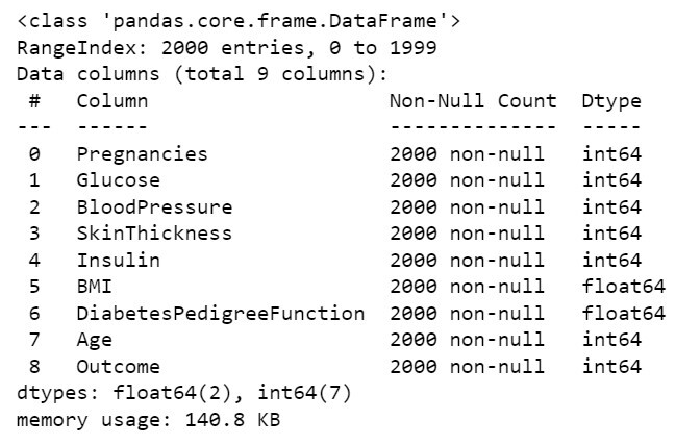
\includegraphics[scale=1.0]{figures/data_info.pdf}
    \caption{Dataset attributes and their data types.}
    \label{fig:capture_a}
\end{figure}
Here, all the attributes in Fig~\ref{fig:capture_a} are numeric and there are no null values. 
\begin{figure}[ht]
    \centering    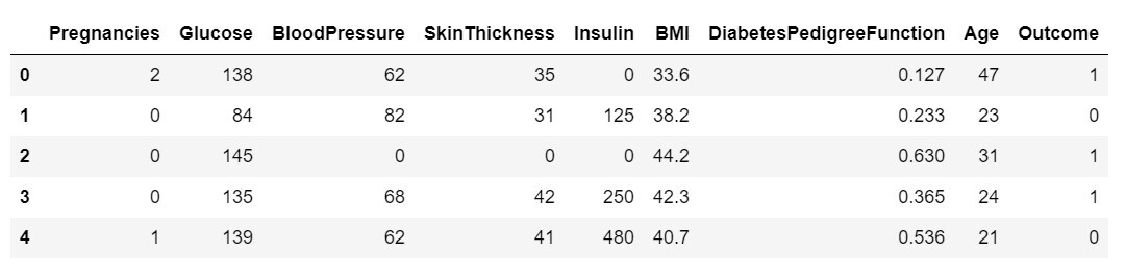
\includegraphics[scale=0.8]{figures/data_top5.pdf}
    \caption{Top 5 patients data.}
    \label{fig:capture_b}
\end{figure}

\subsection{Correlation Matrix}
\label{subsec:corr_matrix}
A correlation matrix is a powerful tool for data analysis. It is a statistical technique used to evaluate the relationship between two variables in a dataset. It provides a correlation coefficient for each cell. The correlation coefficient value remains in the range between -1 and 1.

The correlation coefficient value -1 indicates notable negative linear correlation. The coefficient value 1 indicates notable positive linear correlation. The coefficient value 0 indicates no linear correlation.

A correlation matrix helps summarize data, identify patterns, and make decisions based on relationships between attributes. It helps us to gain insights for building better machine learning models by understanding which attributes are correlated.

\begin{figure}[ht]
    \centering    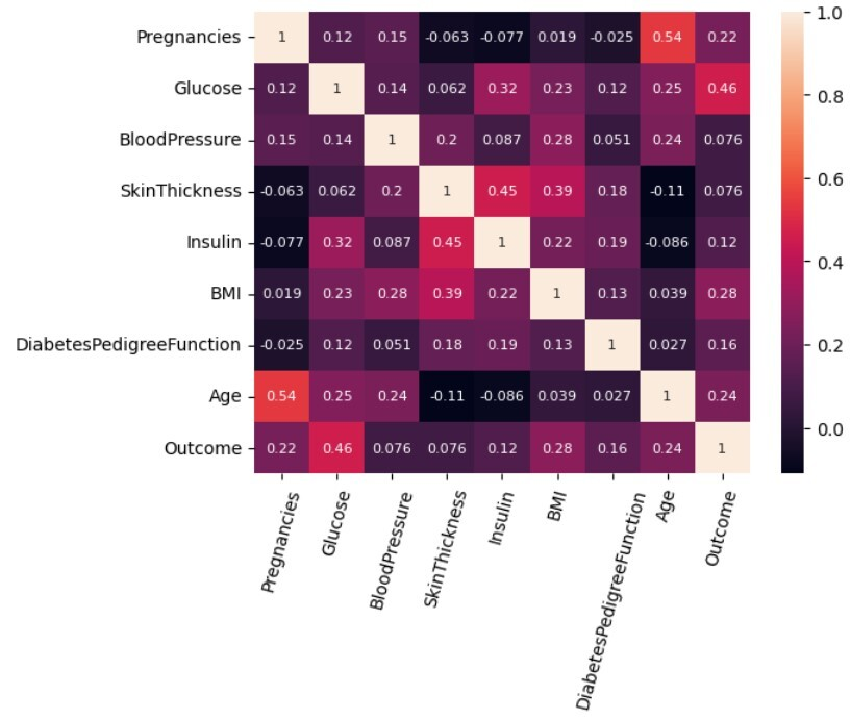
\includegraphics[scale=0.8]{figures/data_correlation.pdf}
    \caption{Correlation Matrix}
    \label{fig:capture_c}
\end{figure}

\subsection{Data Distribution using Histograms}
Fig~\ref{fig:capture_d} gives a better feel than the raw numbers and percentiles of the distributions of our numerical attributes. It shows how each feature and label is distributed along different ranges which further confirms the need for scaling. Next, wherever you see discrete bars, it basically means that each of these is actually a categorical variable. We will need to handle these categorical variables before applying Machine Learning. Our outcome labels have two classes, 0 for no disease and 1 for disease. 
\begin{figure}[ht]
    \centering    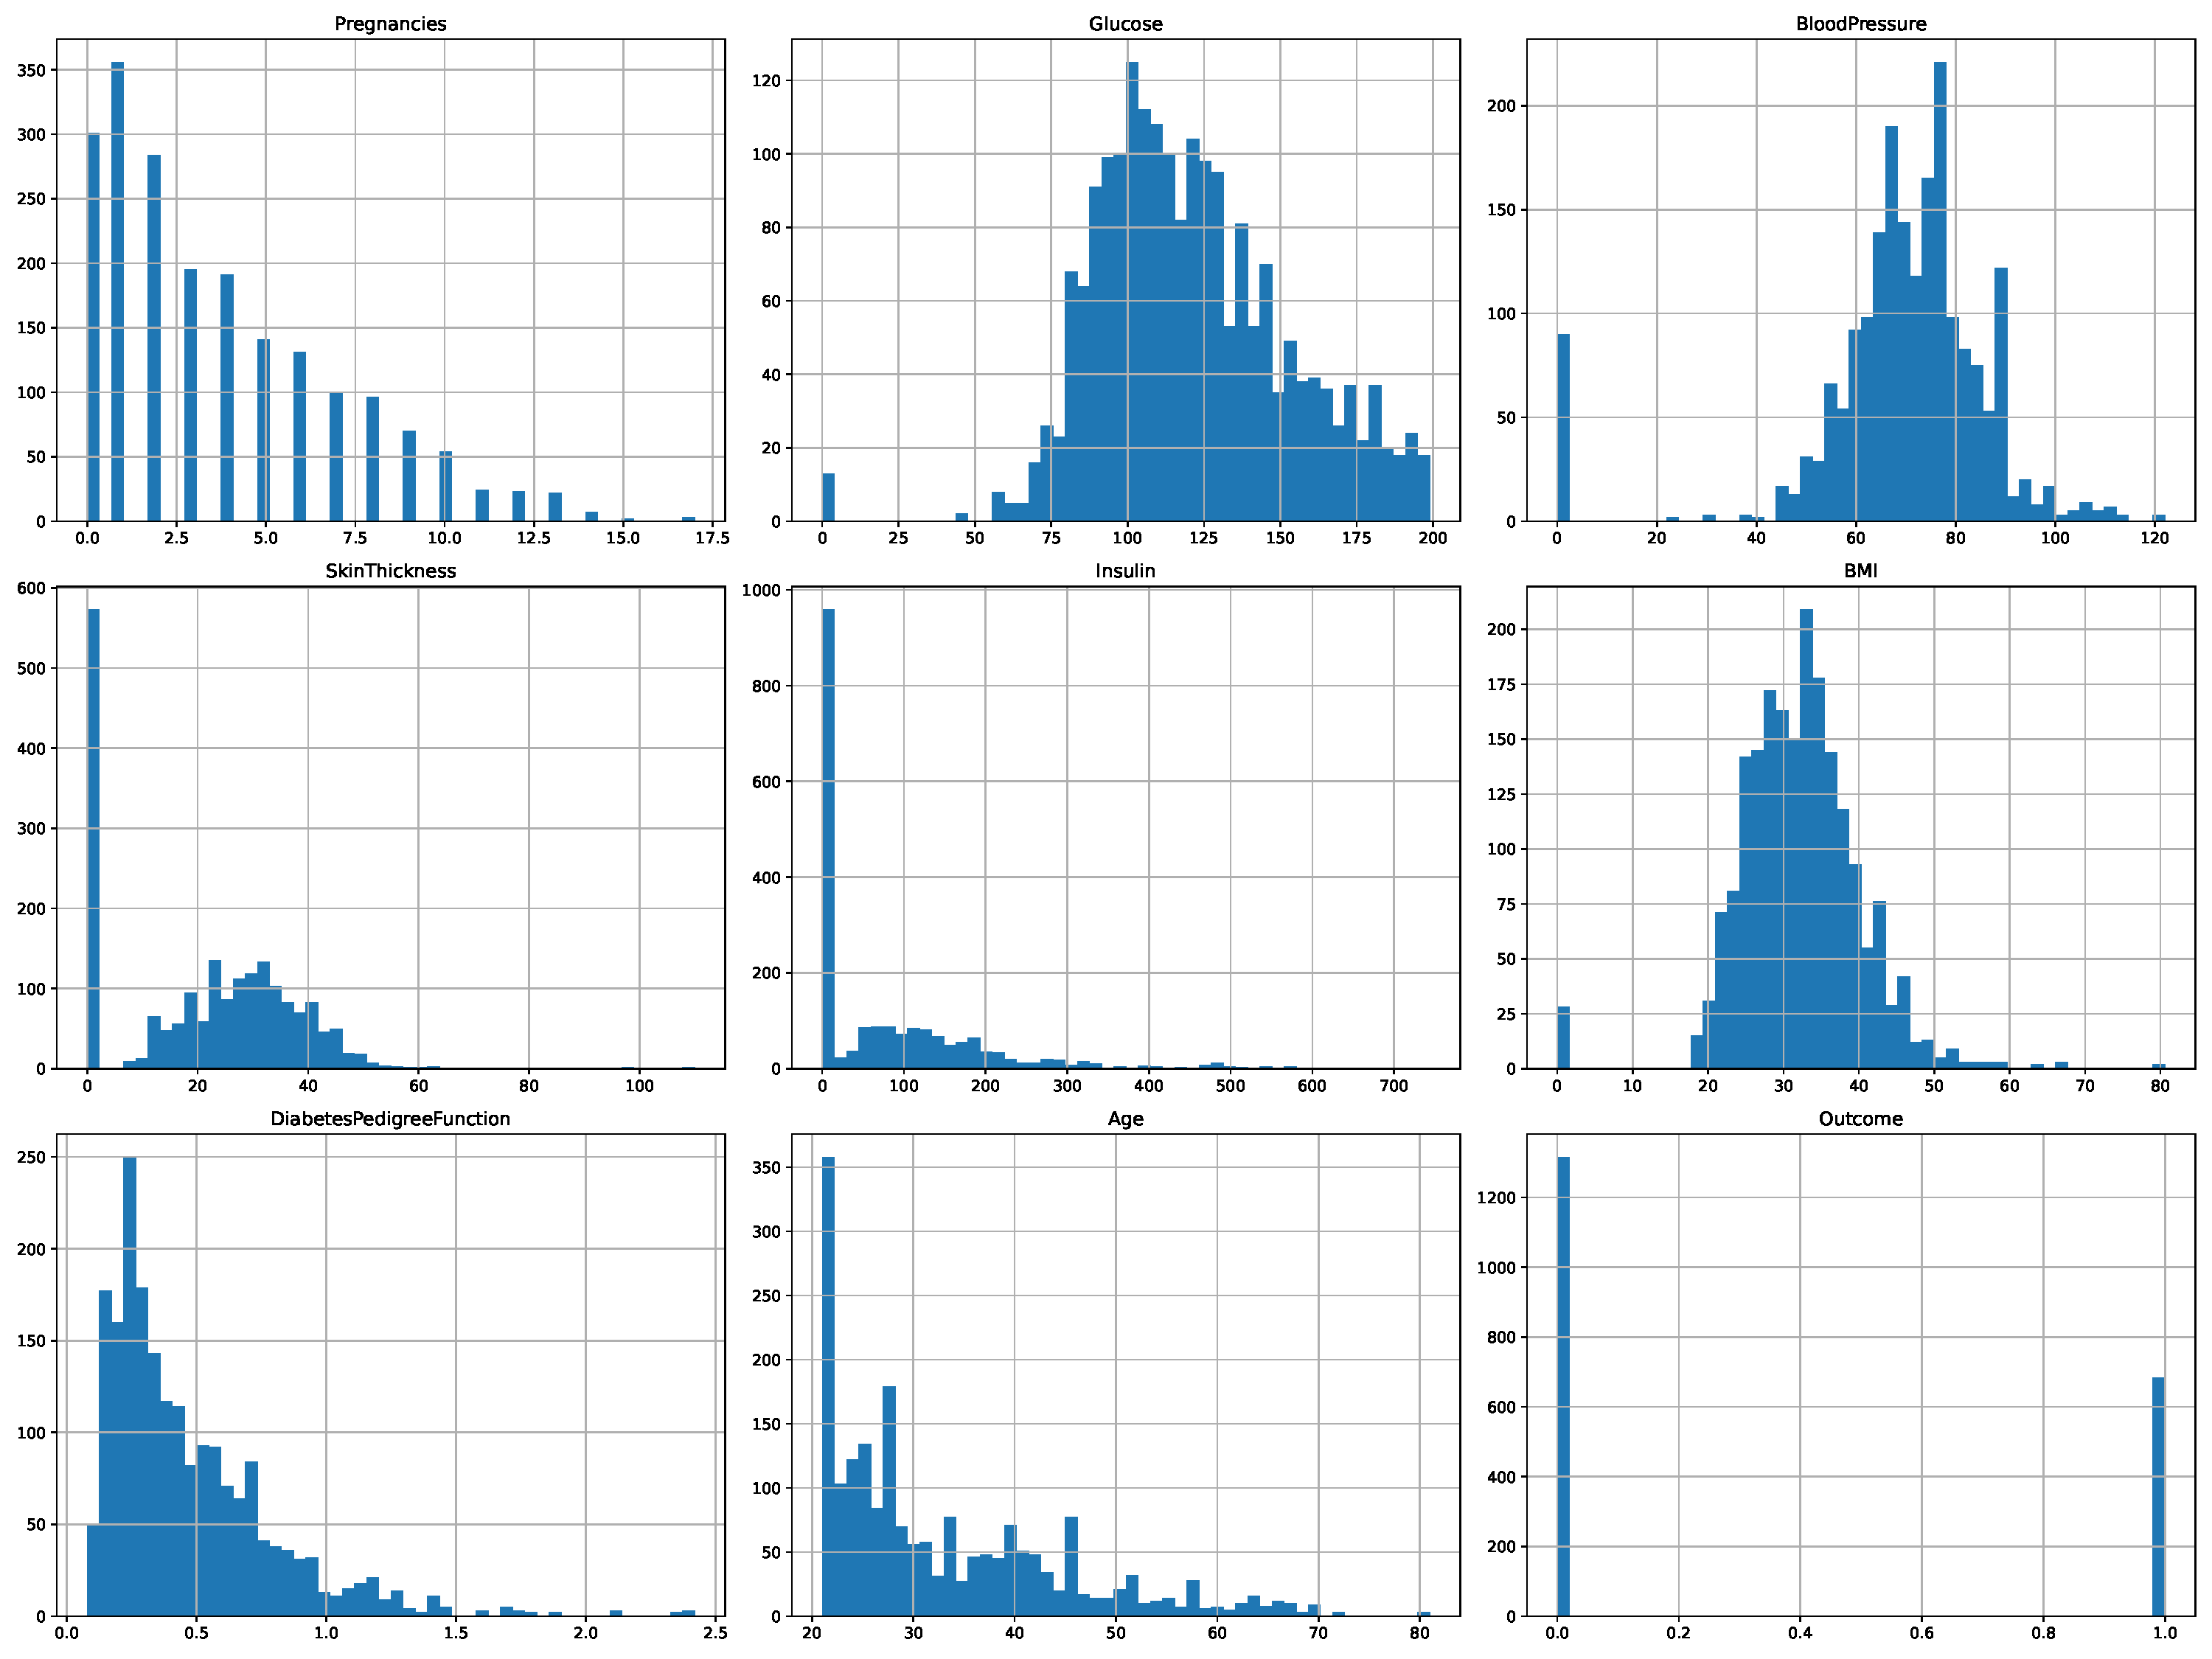
\includegraphics[scale=0.8]{figures/data_attr_distribution.pdf}
    \caption{Data Distribution for each attribute}
    \label{fig:capture_d}
\end{figure}

\subsection{Bar plot for Outcome class}
Fig~\ref{fig:capture_e} shows that the data is biased towards data points having outcome value as 0 which means that diabetes was not present actually. The number of non-diabetics is almost twice the number of diabetic patients.

Out of the 2000 instances, 1316 are associated with non-diabetic patients, while the remaining 684 pertain to diabetic patients.
\begin{figure}[ht]
    \centering    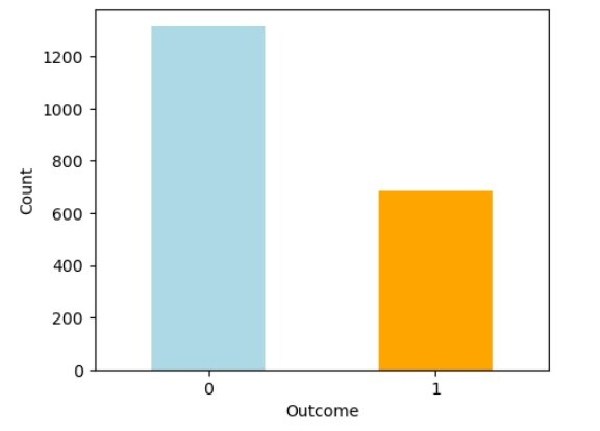
\includegraphics[scale=0.8]{figures/data_distribution.pdf}
    \caption{Distribution of Outcome (0s and 1s)}
    \label{fig:capture_e}
\end{figure}


\section{Data Preprocessing}

Data preprocessing helps to transform data used to built a model which gives higher performance metrics. This process performs various functions like handling missing values, normalization and feature selection to improve the quality of data.

\subsection{Missing Values Identification}
Fig~\ref{fig:capture_a} indicates the absence of null values for all attributes. However, Fig~\ref{fig:capture_b} illustrates instances of zero values for attributes which are irrelevant and need to handled. Table~\ref{tab:table-01-missing-values} shows the number of zero values for each attribute.

 \begin{table}[ht!]
    \centering
    \caption{The number of zero missing values in dataset}
    \begin{tabular}{lrrrrr}
Attributes & No.of missing values (Zero) \\
Pregnancies & 301 \\
Glucose & 13 \\
BloodPressure & 90 \\
SkinThickness & 573 \\
Insulin & 956 \\
BMI & 28 \\
DiabetesPedigreeFunction & 0 \\
Age & 0 \\
\end{tabular}


    \label{tab:table-01-missing-values}
\end{table}

Here, we have observed numerous attributes with zero values, impacting the data quality. We replaced the zero values with the corresponding mean values using simpleimputer.

Fig~\ref{fig:capture_b} and Fig~\ref{fig:capture_f} shows the top five patients data. If you compare these figures, Fig~\ref{fig:capture_f} indicates that zero values in Fig~\ref{fig:capture_b} was replaced with mean for each attribute. Now, there are no missing values either null or zero values in each attribute.

\begin{figure}[ht]
    \centering    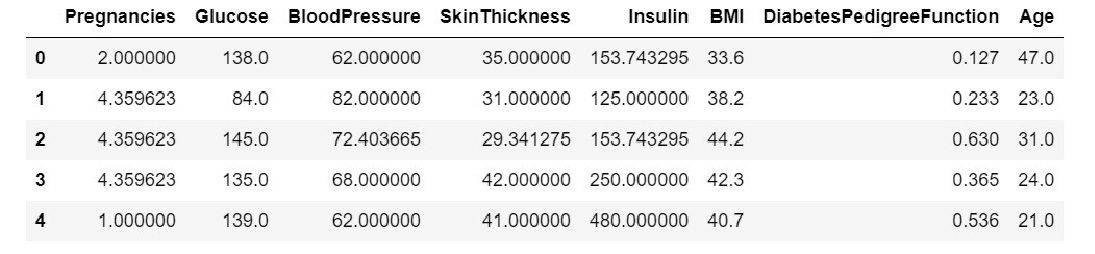
\includegraphics[scale=0.8]{figures/data_info_after_imputer.pdf}
    \caption{Top 5 patients data after handling missing values}
    \label{fig:capture_f}
\end{figure}

\subsection{Feature Selection based on Correlation Coefficient}
After handling missing values, the correlation coefficient is calculated in this method which correlates with the output and input attributes. This was discussed under section~\ref{subsec:corr_matrix}. We have created a Table~\ref{tab:table-02-corr_matrix} to show correlation coefficient values of each attribute towards target attribute.

 \begin{table}[ht!]
    \centering
    \caption{The correlation coefficient values}
    \begin{tabular}{lrr}
 & Correlation Coefficient & Correlation Coefficient after imputation \\
Pregnancies & 0.224437 & 0.249883 \\
Glucose & 0.458421 & 0.488020 \\
BloodPressure & 0.075958 & 0.174481 \\
SkinThickness & 0.076040 & 0.205527 \\
Insulin & 0.120924 & 0.207696 \\
BMI & 0.276726 & 0.282182 \\
DiabetesPedigreeFunction & 0.155459 & 0.155459 \\
Age & 0.236509 & 0.236509 \\
\end{tabular}

    \label{tab:table-02-corr_matrix}
\end{table}

We used 0.2 as a cut-off for relevant attributes. Hence   `BloodPressure` and `DiabetesPedigreeFunction` features are removed. `Pregnancies`, `Glucose`, `SkinThickness`, `Insulin`, `BMI`, and `Age` are our most relevant six input attributes.

\subsection{Data Normalization}
Normalization refers to the process of scaling and transforming numeric features to a standard scale or distribution. Feature scaling is a technique to standardize or normalize the range of independent features or variables of a dataset. The goal of feature scaling is to ensure that all features contribute equally to the learning process, preventing certain features from dominating others based on their scale. In Table~\ref{tab:table-02-corr_matrix}, we can see that `Glucose` and `Outcome` have a 0.49 correlation coefficient. Hence these are highly correlated. After completing data preprocessing, we have total 2000 instances.

\section{Dataset Split into Train and Test Data}
After data cleaning and preprocessing, the dataset becomes ready to train and test. We are using test split method to split data randomly into the training and testing set. Here, I am partitioning the data into a training set comprising 70\% and a test set comprising 30\%.

\section{Model Implementation}
This is the important phase which includes model building for diabetes prediction. In this, we have implemented logistic regression and support vector machine algorithms.

\subsection{Logistic Regression}
Logistic Regression is one of the most common classification models. It is used for classification task where the goal is to predict the probability that an instance belongs to a given class or not. 

\begin{algorithm}
    \caption{Diabetes Prediction using Logistic Regression}
    \label{algo:algo_lr}
    \begin{algorithmic}[1]
        \Require{Input features $X$ and labels $y$ for training data}
        \Ensure{Generate performance metrics like accuracy, confusion matrix, precision, recall, f1-score}
        \Statex
        \State {Create a standard logistic regression model with default hyperparameters such as regularization strength (C), solver, penalty}
        \State {Fit the model with training data}
        \State {Calculate accuracy, confusion matrix, precision, recall and f1-score for the trained model}
        \State {Predict outcomes for testing data using the trained model}
        \State {Evaluate the model performance on testing data}
        \State {Calculate accuracy, confusion matrix, precision, recall and f1-score}
    \end{algorithmic}
\end{algorithm}

\subsection{Support Vector Machine}
Support Vector Machine is used for linear or nonlinear classification, regression, and outlier detection tasks. This classifier aims to establish a hyperplane that can separate the classes by adjusting the distance between data points and the hyperplane. 
\begin{algorithm}
    \caption{Diabetes Prediction using Support Vector Machine}
    \label{algo:algo_svm}
    \begin{algorithmic}[1]
        \Require{Input features $X$ and labels $y$ for training data}
        \Ensure{Generate performance metrics like accuracy, confusion matrix, precision, recall, f1-score}
        \Statex
        \State {Create a standard svm model with default hyperparameters such as regularization parameter (C), kernel, gamma, degree}
        \State {Fit the model with training data}
        \State {Calculate accuracy, confusion matrix, precision, recall and f1-score for the trained model}
        \State {Predict outcomes for testing data using the trained model}
        \State {Evaluate the model performance on testing data}
        \State {Calculate accuracy, confusion matrix, precision, recall and f1-score}
    \end{algorithmic}
\end{algorithm}

\subsection{Hyperparameter Tuning with GridSearchCV}
Hyperparameter Tuning is a process to select optimal values for a machine learning models hyperparameters. The goal of hyperparameter tuning is to find the values that leads to the best performance for a given problem. We should consider the factors like hyper parameters, meta parameter search strategies to achieve more predictive performance metrics.

\subsubsection{Grid Search}
Grid Search is a method for hyper parameter optimization that involves specifying a list of values for each hyper parameter to optimize. Subsequently, the model is trained for each combination of these values, and the optimal values for the hyper parameters are selected based on the models' performance.

\subsubsection{Hyperparameter Tuning for Logistic Regression}
Logistic Regression is one of the most common classification algorithms. It is used for classification task where the goal is to predict the probability that an instance belongs to a given class or not. There are multiple hyper parameters such as regularization strength (C), solver, penalty. We have solvers namely, `lbfgs`, `newton-cg`, `liblinear`, `sag`, `saga`. We have penalties namely, `l1`, `l2`, `elasticnet`, `none`.

\begin{algorithm}
    \caption{Diabetes Prediction using hyperparameter tuning technique for Logistic Regression}
    \label{algo:algo_hp_lr}
    \begin{algorithmic}[1]
        \Require{Input features $X$ and labels $y$ for training data}
        \Ensure{Generate best parameters and calculate performance metrics like accuracy, confusion matrix, precision, recall, f1-score using best parameters}
        \Statex
       \State {Create a standard logistic regression model with no hyperparameters such as regularization strength (C), solver, penalty}
        \State {Create a paramgrid dictionary with all hyperparameters related to logistic regression model you would like to pass to gridsearch for tuning}
        \State {Create a gridsearchcv model by passing parameters such as model estimator, paramgrid, cross validation, scoring methods, refit, verbose}
        \State {Generate the best estimators, best parameters and best scores for training set}
        \State {Calculate accuracy, confusion matrix, precision, recall and f1-score for trained model}
        \State {Predict outcomes for testing data using the trained model}
        \State {Evaluate the model performance on testing data}
        \State {Calculate accuracy, confusion matrix, precision, recall and f1-score}
    \end{algorithmic}
\end{algorithm}

\subsubsection{Hyperparameter Tuning for Support Vector Machine}
This classifier aims at forming a hyper plane that can separate the classes as much as possible by adjusting the 
distance between the data points and the hyper plane. There are several kernels based on which the hyper plane is decided. There are multiple hyper parameters such as regularization parameter (C), kernel, gamma, degree.  We have kernels namely, `linear`, `poly`, `rbf`, and `sigmoid`. 
\begin{algorithm}
    \caption{Diabetes Prediction using hyperparameter tuning technique for Support Vector Machine}
    \label{algo:algo_hp_svm}
    \begin{algorithmic}[1]
        \Require{Input features $X$ and labels $y$ for training data}
        \Ensure{Generate performance metrics like accuracy, confusion matrix, precision, recall, f1-score}
        \Statex
        \State {Create a standard svm model with no hyperparameters such as regularization parameter (C), kernel, gamma, degree}
        \State {Create a paramgrid dictionary with all hyperparameters related to svm model you would like to pass to gridsearch for tuning}
        \State {Create a gridsearchcv model by passing parameters such as model estimator, paramgrid, cross validation, scoring methods, refit, verbose}
        \State {Generate the best estimators, best parameters and best scores for training set}
        \State {Calculate accuracy, confusion matrix, precision, recall and f1-score for trained model}
        \State {Predict outcomes for testing data using the trained model}
        \State {Evaluate the model performance on testing data}
        \State {Calculate accuracy, confusion matrix, precision, recall and f1-score}
    \end{algorithmic}
\end{algorithm}

\section{Summary}
 This methodology provides a structured approach to exploring and showcasing the significance of hyperparameter tuning in enhancing the predictive capabilities of logistic regression and support vector machine models for diabetes prediction. This structured approach encompasses aspects such as dataset characteristics, data exploration, data visualization, preprocessing, normalization, and feature selection to ensure data quality and model design. It delves into data splitting for training and testing, the training of classification models using the training dataset, and the crucial step of hyperparameter tuning to enhance performance metrics by identifying optimal parameters.
 



    \chapter{Results}
\label{ch:results}
\section{Results for ML methods - LR and SVM}
The evaluation of machine learning algorithms is crucial for assessing their effectiveness in predicting diabetes. We use various performance metrics such as accuracy, precision, recall and f1-score to compare the classification methods. These metrics are calculated using equations \ref{eq:accuracy_formula}, \ref{eq:precision}, \ref{eq:recall}, \ref{eq:f1-score}, derived from the confusion matrix.

Table \ref{tab:p_metrics} shows performance measures of logistic regression and svm classifiers for training and testing datasets.

\begin{table}[h!]
    \centering
    \caption{Performance metrics}
    \label{tab:p_metrics}
    \begin{tabular}{llrrrr}     
        \toprule
        Classifier  &   DataSet Type &   Precision   &   Recall  &   F1-score    &   Accuracy (\%) \\
        \midrule
        LR  &   Training    &   0.70   &   0.56   &   0.62    &   77\%   \\
        LR  &   Testing &   0.75   &   0.58   &   0.65    &   79\%   \\
        SVM  &   Training    &   0.76   &   0.71   &   0.74    &   83\%   \\
        SVM  &   Testing &   0.77   &   0.66   &   0.71    &   82\%   \\
        \bottomrule
    \end{tabular}
\end{table}

Here, lr model performed adequately on the training and testing datasets while svm model achieved higher accuracy, with 83\% on the training set and 82\% on the testing set. This higher accuracy, along with better precision, recall, and F1-score, suggests that svm might be a more suitable model for diabetes prediction. The confusion matrix for the svm model on the test dataset is provided in Table \ref{tab:conf_matrix}.

\begin{table}[h!]
    \centering
    \caption{Confusion Matrix for SVM (Test Data)}
    \label{tab:conf_matrix}
    \begin{tabular}{llr}     
        \toprule
        & Diabetic  &   Non-diabetic \\
        \midrule
        Diabetic &  236  &   27   \\
        Non-diabetic &  46    &   91  \\
        \bottomrule
    \end{tabular}
\end{table}

Despite these promising results, determining the best model for predicting diabetes requires further investigation and analysis.

\section{Hyperparameter Tuning Results for LR and SVM Using GridSearchCV}
After applying gridsearchCV for hyperparameter tuning, both logistic regression and svm models demonstrated significantly improved performance compared to their standard configurations which was shown in Table \ref{tab:p_metrics}. 

Table \ref{tab:gs_p_metrics} shows performance measures of logistic regression and svm classifier for training and testing datasets after tuning.

\begin{table}[h!]
    \centering
    \caption{Performance metrics after hyperparameter tuning}
    \label{tab:gs_p_metrics}
    \begin{tabular}{llrrrr}     
        \toprule
        Classifier  &   DataSet Type &   Precision   &   Recall  &   F1-score    &   Accuracy (\%) \\
        \midrule
        LR  &   Training    &   0.72   &   0.54   &   0.62    &   77\%   \\
        LR  &   Testing &   0.80   &   0.57   &   0.67    &   81\%   \\
        SVM  &   Training    &   0.79   &   0.76   &   0.77    &   85\%   \\
        SVM  &   Testing &   0.78   &   0.66   &   0.72    &   82\%   \\
        \bottomrule
    \end{tabular}
\end{table}

Hyperparameter tuning significantly improved both models' performance. Here, svm model achieved the highest accuracy 85\% on the training dataset and 82\% on the testing dataset. LR model also saw improvements, with 81\% testing accuracy. While both models showed good precision, the recall could still be enhanced. Fine-tuning hyperparameters led to improved overall accuracy and balanced performance. However, further refinement may be needed to increase recall and reduce misclassifications. The confusion matrix for the svm model on the test dataset is provided in Table \ref{tab:gs_conf_matrix}

\begin{table}[h!]
    \centering
    \caption{Confusion Matrix for SVM (Test Data)}
    \label{tab:gs_conf_matrix}
    \begin{tabular}{llr}     
        \toprule
        & Diabetic  &   Non-diabetic \\
        \midrule
        Diabetic &  238  &   25   \\
        Non-diabetic &  46    &   91  \\
        \bottomrule
    \end{tabular}
\end{table}

The optimized models achieved higher accuracy scores, highlighting the effectiveness of hyperparameter tuning in enhancing predictive capabilities.

\section{Summary}
The evaluation of machine learning algorithms lr and svm for predicting diabetes demonstrated promising results. Although both models had comparable performance on the training dataset, svm outperformed lr on the testing dataset, achieving 82\% accuracy. Hyperparameter tuning with gridsearchCV further improved the models' performance, with the optimized svm achieving an accuracy of 82\% on the testing set, highlighting the effectiveness of this technique. These results suggest that svm might be more effective for diabetes prediction, but additional tuning and exploration could further enhance the performance of both models. These findings underscore the effectiveness of hyperparameter tuning in improving predictive capabilities.




    \chapter{Discussion and Analysis}
\label{ch:evaluation}

Depending on the type of project you are doing, this chapter can be merged with ``Results'' Chapter as `` Results and Discussion'' as suggested by your supervisor. 

In the case of software development and the standalone applications, describe the significance of the obtained results/performance of the system. 



\section{A section}% please use an appropriate section title
Discussion and analysis chapter evaluates and analyses the results. It interprets the obtained results. 



\section{Significance of the findings}
In this chapter, you should also try to discuss the significance of the results and key findings, in order to enhance the reader's understanding of the investigated problem

\section{Limitations} % please discuss limitation of the project 
Discuss the key limitations and potential implications or improvements of the findings.
\section{Summary}
Write a summary of this chapter.
    \chapter{Conclusions and Future Work}
\label{ch:con}
\section{Conclusions}
Early detection of diabetes is one of the significant challenges in the health care industry. Our research delved into the realm of diabetes prediction using logistic regression and support vector machines models, aiming to shed light on their comparative performance metrics and underlying factors. 

In our research, we designed a system which can predict diabetes with high accuracy. We preprocessed the data by addressing missing values, zero-valued features, and employing imputation techniques across all features. Using the feature reduction method, we dropped two features. We used six input features - `Pregnancies`, `Glucose`, `SkinThickness`, `Insulin`, `BMI` and `Age` and one output feature `Outcome` in the  dataset \citep{dataset}. We explored the efficacy of two machine learning algorithms, lr and svm to predict diabetes and evaluated the performance on various measures like accuracy, precision, recall, and f1-score. These models provided an accuracy greater than 70\%.

Furthermore, our exploration of hyperparameter optimization strategies underscores the importance of fine-tuning model parameters to achieve optimal predictive performance. To enhance model performance, we employed hyperparameter tunning using gridsearchCV strategy, optimizing parameters. These models provided good accuracy before tuning and svm outperformed lr for both train/test split method. After tuning, the optimized models exhibited notable improvements in accuracy, with svm achieving an impressive accuracy of approximately 82\% on the test dataset. while lr slightly trailing behind, still demonstrated commendable performance, boasting an accuracy close to 81\%.

\section{Future work}
The results from Chapter~\ref{ch:results} indicate that both logistic regression and support vector machine classifiers achieved reasonable performance in predicting diabetes, with svm attaining slightly higher accuracy. However, there are several areas for future research that can further enhance the predictive capabilities of these models and address their limitations.

\begin{itemize}
\item A critical aspect for future work is the expansion of the dataset. The current study dataset may not fully represent the diverse population affected by diabetes. Increasing the dataset's size and diversity would improve the model's generalizability and robustness. It would also help reduce biases and ensure that the models work across different demographics and geographic locations.

\item Future studies can delve into additional feature engineering techniques. By incorporating domain-specific knowledge from medical professionals and using automated feature selection methods like recursive feature elimination, new features may be uncovered that contribute significantly to prediction accuracy. This approach could also lead to more refined models with reduced risks of overfitting.

\item Future work could explore more complex architectures such as deep neural networks (DNNs), convolutional neural networks (CNNs), and recurrent neural networks (RNNs). These models might capture intricate patterns in the data that traditional machine learning models might miss. Deep learning methods could improve prediction accuracy and add robustness to the models.

\item Another crucial aspect for future work is managing class imbalances. Class imbalance in the dataset can lead to biased models and high false negatives. Techniques like oversampling, undersampling, and Synthetic Minority Over-sampling Technique (SMOTE) could be used to balance the classes, resulting in improved recall and better model performance.

\item The current study utilized gridsearchCV for hyperparameter tuning, other methods such as randomizedsearchcv and bayesian optimization offer more flexible and efficient tuning processes. Future work could investigate these methods to optimize model performance further, potentially achieving higher accuracy and reliability.

\item Integrating these models into clinical practice is a valuable future direction. Building a user-friendly interface for healthcare professionals and conducting clinical trials would be essential to validate the models' effectiveness in real-world. This step is crucial for demonstrating that these models can assist in early diabetes diagnosis and improve patient outcomes.
\end{itemize}

    \chapter{Reflection}
\label{ch:reflection}
%%%%%%%%%%%%%%%%%%%%%%%%%%%%%%%
%% Please remove/replace text below
%%%%%%%%%%%%%%%%%%%%%%%%%%%%%%%
Write a short paragraph on the substantial learning experience. This can include your decision-making approach in problem-solving.

\textbf{Some hints:} You obviously learned how to use different programming languages, write reports in \LaTeX and use other technical tools. In this section, we are more interested in what you thought about the experience. Take some time to think and reflect on your individual project as an experience, rather than just a list of technical skills and knowledge. You may describe things you have learned from the research approach and strategy, the process of identifying and solving a problem, the process research inquiry, and the understanding of the impact of the project on your learning experience and future work.

Also think in terms of:
\begin{itemize}
    \item what knowledge and skills you have developed
    \item what challenges you faced, but was not able to overcome
    \item what you could do this project differently if the same or similar problem would come
    \item rationalize the divisions from your initial planed aims and objectives.
\end{itemize}


A good reflective summary could be approximately 300--500 words long, but this is just a recommendation.

~\\[2em]
\noindent
{\huge \textbf{Note:}} The next chapter is ``\textbf{References},'' which will be automatically generated if you are using BibTeX referencing method. This template uses BibTeX referencing.  Also, note that there is difference between ``References'' and ``Bibliography.'' The list of ``References'' strictly only contain the list of articles, paper, and content you have cited (i.e., refereed) in the report. Whereas Bibliography is a list that contains the list of articles, paper, and content you have cited in the report plus the list of articles, paper, and content you have read in order to gain knowledge from. We recommend to use only the list of ``References.'' 

    

    
    % -------------------------------------------------------------------
    % Bibliography/References  -  Harvard Style was used in this report
    % -------------------------------------------------------------------
    \bibliographystyle{agsm} % Harvard Style 
    
    \bibliography{references}  %  Patashnik, O. (1988), BibTEXing. Documentation for general BibTEX users.
    
    % -------------------------------------------------------------------
    % Appendices
    % -------------------------------------------------------------------
    
    \begin{appendices}
        \chapter{An Appendix Chapter (Optional)}
\label{appn:A}
% Optional chapter
Some lengthy tables, codes, raw data, length proofs, etc. which are \textbf{very important but not essential part} of the project report goes into an Appendix. An appendix is something a reader would consult if he/she needs extra information and a more comprehensive understating of the report. Also, note that you should use one appendix for one idea.

An appendix is optional. If you feel you do not need to include an appendix in your report, avoid including it. Sometime including irrelevant and unnecessary materials in the Appendices may unreasonably increase the total number of pages in your report and distract the reader.


        \chapter{An Appendix Chapter (Optional)}
\label{appn:B}

...
    \end{appendices}
    
\end{document}
